% !TeX encoding = UTF-8
% !TeX program = xelatex
% !TeX spellcheck = <none>

\documentclass[degree=master,cjk-font=noto]{thuthesis}
% 著者-出版年制
\usepackage[sort]{natbib}
\bibliographystyle{thuthesis-numeric}
\usepackage{mathtools}
\usepackage{tikz}
\usetikzlibrary{shapes,arrows}
\usepackage[autosize]{dot2texi}
% Syntax Highlighting in LaTeX, need pygments
% Must build with xelatex -shell-escape -enable-8bit-chars.
\usepackage{minted}
% https://tex.stackexchange.com/a/112573
\usepackage{tcolorbox}
\usepackage{etoolbox}
\BeforeBeginEnvironment{minted}{\begin{tcolorbox}}%
\AfterEndEnvironment{minted}{\end{tcolorbox}}%
% color for minted
\definecolor{friendlybg}{HTML}{f0f0f0}

\usepackage{multirow}
\usepackage{rotating}

% 论文基本配置,加载宏包等全局配置
\thusetup{
    output = electronic,
    title  = {基于注意力机制的序列模型在网络流量分类及保护上的应用},
    author  = {肖文韬},
    studentid = {2020214245},
    major = {电子信息(计算机技术)},
    email = {xwt20@mails.tsinghua.edu.cn},
    course = {开题报告},
    include-spine = false,
}

\usepackage{float}
\graphicspath{{figures/}}


\begin{document}

% 封面
\maketitle

\frontmatter
\begin{abstract}
  不需要。

  \thusetup{
    keywords = {流量分类, 注意力机制, 序列模型, GAN},
	}
\end{abstract}

\begin{abstract*}
  No need.

  % Use comma as seperator when inputting
  \thusetup{
    keywords* = {Recommendation System, click-through rate, deep learning, xDeepFM, AutoInt, FGCNN},
  }
\end{abstract*}


% 目录
\tableofcontents

% 插图和附表清单
\listoffiguresandtables
% \listoffigures           % 插图清单

% 正文部分
\mainmatter

\chapter{研究背景和意义}

\section{研究背景}

网络流量分析是一个完整的过程,从拦截流量数据开始,到发现互联网网络中的关系、斑点、异常和错误配置,以及其他事项。
特别是,流量分类是该领域策略的一个子组,其目的是根据用户的要求,将互联网流量分为预定义的类别,如正常或异常流量、应用程序的类型(流媒体、网络浏览、VoIP等)或应用程序的名称(YouTube、Netflix、Facebook等)。
网络流量分类在保证网络安全和网络系统稳定运行方面发挥着重要作用,引起了学术界和工业界的广泛关注。
网络流量分类之所以很重要,是因为有以下几个原因:
a) 故障排除任务:主要目的是定位有问题的网络设备、设备/软件的错误配置、定位数据包丢失点、网络错误等。
在这个领域,识别或分类网络中的应用程序的名称或类型,有助于处理一些事先的问题。
b) 安全性:避免恶意软件或防止对私人信息的入侵。
c) 服务质量(QoS)管理,以保证终端用户对应用或服务的总体接受度。
例如,从流量中识别不同的应用,对于管理带宽资源和确保QoS要求至关重要。

在过去,流量分类依赖于基于端口的方法,即每个应用程序通过其注册的和已知的端口来识别,这些端口由互联网分配号码管理局(IANA)定义。
这种方法现在已经变得不可靠和不准确,因为除其他因素外,具有未注册或随机生成的端口的新应用程序的扩散。
另一种在该领域获得大量普及的方法被称为深度包检测(DPI)。
DPI在数据包有效载荷和存储的签名集之间进行匹配,以对网络流量进行分类。
然而,当隐私政策和法律阻止访问数据包内容时,以及在协议混淆或封装的情况下,DPI会失败。
为了克服前述问题,机器学习成为一个合适的解决方案,不仅适用于流量分类任务,还适用于预测和新知识发现等~\cite{net2,net3,app_class,SDN_HGW,DMTCS,bitcoding}。
在这种情况下,网络流量的统计特征通常从网络流中提取出来,并存储起来以生成历史数据。
通过这种方式,可以用这些历史数据来训练不同的机器学习模型,并且可以用这些模型来分析新进入的流量。
这些方法首先在数据包层面或流量层面提取特定协议的特征,然后使用这些特征来构建流量分类的分类器。在数据包层面,每个数据包都将被分类。
在流量层面上,分类的粒度是流量。
各种有监督和无监督的方法已经被用来对许多网络协议进行分类。
然而,这些方法面临两个挑战性的问题。首先,由于存在巨大的新应用,手工寻找对所有应用都有效的新特征是很耗时和容易出错的。
其次,现代应用的网络流量是如此的复杂和动态,以至于传统的挖掘方法不能很好地概括出特定应用的准确指纹。
为了解决这些挑战,在本课题中,我们使用基于注意力机制的序列模型来自动地学习网络流量的表示。
我们提出的序列模型能够学习出更复杂、更具表达性的特征,同时能够带来较好的泛化性能和鲁棒性。

近十年来我国的互联网行业一直走在世界的前列,各式各样的信息科技创新模式和技术在我国互联网行业内生根发芽,且正以不可思议的速度发展。
跟随互联网的发展和大数据科技的快速崛起,国内外的应用程序和网站呈现爆发式的增长。
截至 2021 年 6 月~\cite{CNNIC-report},我国三家基础电信企业的移动电话用户总数达 16.14 亿户,较 2020 年 12 月净增 1985 万户。
其中,5G 手机终端用户达 3.65 亿户,较 2020 年 12 月增加 1.66 亿户。
截至 2021 年 6 月,我国网民规模达 10.11 亿,其中手机网民规模达 10.07 亿,较 2020 年 12 月增长 2092 万,网民使用手机上网的比例为 99.6\%。
互联网给人们提供了越来越多的个性化资讯,并在工作、娱乐,生活中服务于大众,受到了人们的欢迎。
在这一庞大的用户体量下,各种应用程序和网站的需求呈现爆发式增长。
截至 2021 年 6 月,我国国内市场上监测到的应用程序数量为 302 万款,而且每天都会有一大批新的应用程序出现。
截至 2021 年 6 月,我国网站数量为 422 万个。

科技是把双刃剑,互联网给人们生活带来便利的同时,也受到了恶意攻击者的关注。
如今不管是应用程序还是网站大多存在安全隐患。
以 Android 应用程序为例,根据移动互联网系统与应用安全国家工程实验室和爱加密移动应用大数据平台提供的数据,截止 2021 年 9 月底大数据平台共计收录 Android 移动应用程序 347 万款,其中 70\% 以上存在高危漏洞威胁~\cite{App-report},这类应用程序容易遭受不同形式的攻击。
据调查,几乎所有(89\%)的漏洞都可以被恶意软件利用~\cite{ZOL-report}。
正由于目前的应用程序漏洞总量特别庞大,这就有让黑客窃取个人密码、金融信息或隐私数据的可能。
如多数应用程序存在滥用各类共享权限的情况,容易被不法分子利用,导致隐私的泄露。
通过应用程序发起恶意攻击的攻势越来越猛烈。
据统计,每年至少新增 150 万种恶意移动软件,至少造成超过 1600 万件的恶意移动软件攻击事件~\cite{Attack-report}。

2021 年 4 月,全球领先的网络安全解决方案提供商 Check Point® 软件技术有限公司发布了《2021 年移动安全报告》~\cite{Attack2-report}。
报告全面概述了移动恶意软件、设备漏洞及国家级网络攻击的趋势,并介绍了如何抵御当今和未来复杂的移动威胁。
报告显示,2020 年,几乎每个组织都经历了至少一次移动恶意软件攻击。
这些攻击中有 93\% 源于互联网,它们试图诱骗用户通过受感染的网站或网址安装恶意应用,或者窃取用户凭据。
46\% 的组织至少有一名员工下载了威胁网络和数据的恶意应用。
由于芯片组的缺陷,全球至少有 40\% 的移动设备存在固有的漏洞,需要紧急打补丁。
目前全世界正处于新冠疫情的影响之下,这些恶意软件通常会隐藏在生成提供疫情相关信息的应用中。
诸如此类的应用程序用户可能遭受不同形式的恶意攻击,包括网络流量分类攻击以及通过恶意应用程序攻击来窃取用户的个人隐私或者个人财产。
所以针对利用网络流量分类的攻击,我们需要使用网络流量保护技术来抵御这些攻击。

\section{研究意义}

综上所述,网络流量分类发挥着重要重要,但是已有的方法无法适应现在越来越复杂和动态的网络环境,这促使我们研究基于注意力机制的序列模型来进行高效、高精度地网络流量分类方法。
在看似和谐的网络社会中,隐藏着众多危害社会安全和健康的内容,比如赌博、色情网站等国家明令禁止的社会活动。最高人民法院、最高人民检察院、公安部日前联合出台了《关于办理网络赌博犯罪案件适用法律若干问题的意见》~\cite{intro-9},明确表示利用互联网、移动通讯终端等传输赌博视频、数据,组织网络赌博等是犯罪行为。在全国扫黄行动中,明确了色情内容是网络违法犯罪活动~\cite{intro-10}。今年9月24日国家发改委、央行等10余个部委联合发布通知~\cite{intro-11},对虚拟货币“挖矿”和交易炒作进行全面整治和打击,把虚拟货币“挖矿”定性为违法。可见,这些特殊的应用场景或者用户行为将极大的影响网络健康发展以及社会秩序。从体量庞大的软件生态中甄别这些恶意应用或恶意行为,成为了目前网络社会十分急切的需求。
因此恶意应用程序和网站的检测技术对于社会的健康发展来说意义非凡。特别的是,当前新冠疫情常态化,远程办公方式大规模兴起,网络攻击面急剧扩大,97\% 的组织面临着来自多个方面的移动威胁。据预测,到2024年将有 60\% 的员工转向移动办公方式,使用网络流量分类技术保障网络流量安全成为所有组织的当务之急。


同时,攻击者也能使用网络流量分类技术来进行攻击,尤其是在公司和政府机构建立的一些涉密信息的网络传输通道中,用户使用的应用程序和访问的网站信息一旦被泄露,可能造成严重后果。
攻击者使用网络流量分类技术盗取用户的敏感隐私信息,利用这些信息对用户产生严重的威胁。最近,人们对隐私信息的泄漏越来越重视,政府制定了多条法律保障用户的隐私。例如,香港制定了《个人资料(私隐)条例》,中国大陆制定了《中华人民共和国网络安全法》和《中华人民共和国个人信息保护法》,欧盟实施了通用数据保护条例 (GDPR)。
为了抵御这类攻击,在本研究中我们也将探索基于注意力机制的序列模型来对网络流量进行保护,使得攻击者攻击失败。


\chapter{国内外研究现状}

\section{网络流量分类}

学术界关于网络流量分类的研究采用了很多种不同的技术。在本节中,我们主要关注基于机器学习的方法。尽管越来越多的应用程序使用SSL/TLS来保护他们的流量,但仍有大量的信息可以从加密的流量中得知,如数据包的长度、方向、元数据和TCP时间戳。我们把这种信息称为侧信道数据。同时,有效载荷内容也在从网络流量中获取有用信息方面发挥着重要作用,即使它们是加密的。根据流量分类中使用的信息,这些方法可分为两类。1)基于侧信道数据的方法,和2)基于有效载荷内容的方法。

\subsection{基于侧信道数据的方法}


基于旁路数据的方法主要采用数据包头和流量的信息。典型的侧信道数据包括根据流量中的源和目标IP地址的数据包长度和方向等。整个网络流量中的侧信道数据序列也包含有用的信息。因此,现有的研究通常首先获取侧信道数据序列,然后将其转化为适合机器学习的特征~\cite{app_class}。特别是,可以从侧信道数据中提取两类特征用于流量分类。

\subsubsection{统计特征}


许多统计数据可以从侧通道数据序列中获得,包括计数、最大、最小、平均、标准差、方差、倾斜、中位绝对偏差、峰度、百分比等。这些数字是由整个流或子流计算出来的。一个子流程是具有某些约束的流程的一部分。例如,突发是一种子流,由方向相同的连续数据包组成~\cite{SSFW10}。Roughan等人使用最近的邻居、线性判别分析和二次判别分析方法,根据统计数据对流量进行分类~\cite{b11}。Bernaille等人观察到,TCP连接的前几个数据包的大小和方向很重要。根据这一观察,他们提出了一个基于简单K-means的模型~\cite{b12}。有许多基于集群技术的方法。Zhang等人~\cite{b15}利用流量相关信息,通过流量标签传播和包括K-means聚类在内的复合分类技术来识别未知应用。Luis Sacramento等人~\cite{flowhacker}在进行聚类时发现,恶意流量位于真实流量中的小聚类,并实现了一个名为FlowHacker的新型网络入侵检测系统(NIDS)。他们的方法从流量中自动提取特征并利用两阶段聚类来迭代检测攻击。

此外,Taylor等人实现了一个应用分类框架~\cite{app_class},它利用数据包长度序列的统计特征,对智能手机应用进行指纹识别。他们评估了其在不同设备、应用程序版本和时间上的鲁棒性。最近,在区块链的新兴领域~\cite{chen2019tokenscope,EOS20},如智能合约和去中心化的应用程序,Shen等人~\cite{DApps}识别了以太坊~\cite{8486401}上的去中心化应用程序(DApps)的加密流量。他们通过利用多项式和径向基等核函数,融合了三个不同维度的统计特征(即数据包长度、突发和时间序列)。对于数据包长度,Kampeas el at.提出了一种有效的采样策略~\cite{zero_length},以满足软件定义网络(SDN)环境中的实时分类需求,该策略只使用有效载荷长度为零的数据包,如TCP流中的ACK,以恢复整个数据包长度序列。他们利用流量中的前 $k$ 个a-APDUs作为特征,其中a-ADPU是在同一方向传输的连续数据包的数据字节长度之和。

\subsubsection{序列特征}

同一流量中的数据包之间的关系信息在网络流量分类中也起着至关重要的作用。由于侧信道数据可以从加密的网络流量中提取并形成时间序列,因此使用基于马尔可夫模型的方法自然是合适的。Anderson等人~\cite{kdd_encrypted_malware}利用三种特征对加密的恶意软件流量进行了二元分类:长度和时间的统计特征、由流量的前50个数据包的大小构建的一阶马尔可夫链以及TLS握手元数据的特征。随后,多属性马尔可夫概率指纹(MaMPF)在~\cite{MaMPF}中被提出。作者发现,数据包的长度是受幂律分布影响的。因此,他们首先采用幂律划分,将数据包长度序列转化为更具辨识度的长度块序列(LBS)。然后,为消息类型序列(MTS)和LBS建立了两个马尔可夫模型。最后,这些模型的输出概率被送入机器学习分类器。

由于循环神经网络(RNN)适合于序列数据的建模,Liu等人设计了一个新的深度学习模型,名为流量序列网络(FSNet)~\cite{fsnet},用于使用数据包长度序列的加密流量级分类。FS-Net利用自动编码器架构与重建机制来促进特征学习,其中编码器和解码器都是两层Bi-GRU。

\textbf{总结}:大多数现有的方法都是基于从数据包头中提取的特定侧信道特征建立模型。为了利用更粗略和更广泛的侧信道特征,而不是现有研究中使用的手工制作的特征,我们的模型从网络流量中自动学习最合适的侧信道特征。

\subsection{基于有效载荷内容的方法}

数据包的有效载荷可被视为一串字节或比特。为了利用有效载荷提供的信息,传统方法试图找到与网络流量相匹配的签名。这些签名通常是 $n$-grams或关键词的形式,网络流量的识别利用了有效载荷中签名的出现频率。除了这些传统的基于签名的方法,自然语言处理(NLP)的技术,如主题模型也被使用。同时,深度学习也被引入,以学习复杂但有用的数据包的表示。

\subsubsection{基于签名的方法}

基于签名的方法使用从有效载荷中提取的签名从网络流量中识别应用协议。Deri等人开发了一个开源的高速深度包检测工具,名为nDPI~\cite{b24},它支持超过 $500$ 种不同的协议。通过使用从数据包头和有效载荷中提取的字节级的签名,DPI可以在不降低网络吞吐量的情况下进行流数据中的字符串检测。它取得了很高的准确性和效率,但需要对每个协议有预先的了解。为了克服这一限制,Hubballi等人提出了一种基于比特级DPI的签名构建方法,称为BitCoding~\cite{bitcoding}。为了自动匹配所有具有相同标签的样本的比特序列(即数据包有效载荷的内容),他们使用数据包中有效载荷的前 $k$ 比特(如果第一个数据包的长度小于 $k$ 比特,则使用流),从计数中产生一个压缩的签名。该签名与正则表达式类似,只有三个运算符,即 $.$、$*$ 和 $\{n\}$。他们还使用Relaxed Hamming Distance~\cite{bitcoding}来测量签名的重叠度,可以通过增加 $k$ 来减少。

此外,Haffner等人利用三种机器学习算法,即Naive Bayes、AdaBoost和Maximum Entropy,从TCP流的前 $n$ 个字节中自动提取签名~\cite{b19}。

\subsubsection{基于主题模型的方法}

由于NLP中的词-文档关系和网络流量中的字节-负载关系的相似性,一些研究使用自然语言处理(NLP)中的主题模型技术来寻找网络流量分类的有力关键词。主题模型的目的是发现文档的抽象关键词。同样地,一些研究人员致力于寻找通用的关键词来识别网络流量中的数据包。Securitas~\cite{b25}是第一个基于主题模型的方法,它应用Latent Dirichlet Allocation(LDA)和词包模型来提取协议的特征。该特征是具有相同协议的有效载荷中的关键词的分布。然后,采用支持向量机(SVM)、C4.5决策树或贝叶斯网络来做分类。此外,Xiao等人~\cite{DMTCS}使用动态集群主题模型来获得集群中最常见的关键词,用于流量分类模型。

\subsubsection{基于深度学习的方法}

深度学习已经被广泛应用于许多重要领域,包括流量分类和网络攻击检测~\cite{iot_attack_detection}。在智能家居软件定义网络(SDN)的场景中,Wang等人提出了一个受SDN启发的家庭网关框架(SDN-HGW)~\cite{SDN_HGW},提供细粒度的应用级流量分类。他们开发了名为DataNets的加密数据分类器,该分类器由三个虚构的深度学习模型组成,即多层感知器、卷积神经网络(CNN)和堆叠的自动编码器。同时,Lotfollahi等人提出了DeepPacket~\cite{deep_packet},具有类似的深度学习模型。一维(1D)CNN是在他们的实验中取得最佳性能的拟议模型之一。它将一维字节矢量化的数据包转化为二维的张量。Giuseppe Aceto等人利用多模态深度学习~\cite{MIMETIC}和融合~\cite{mobile_app_class}技术来提高性能。这些模型要么错过了网络流量的特点,要么涉及许多高开销模块,引入了不必要的计算开销。因此,我们设计了一个新颖的神经网络,它适合网络流量的特点,并且从实验结果来看,它的性能优于DeepPacket~\cite{deep_packet}。

\textbf{总结}:与基于侧信道数据的方法相比,基于有效载荷内容的方法涉及更多流量信息,即数据包的有效载荷内容。由于网络流量行为的复杂性,传统的机器学习方法很难提取特征。我们设计了一种新颖的基于深度学习的流量分类方法,不需要提取特征。

\section{网络流量保护}

网络流量保护系统对数据包进行修改(增加数据包或负载、延迟或重路由),以防止使用攻击者使用网络流量分类技术分析网络流量。
广义上讲,这些保护措施要么是根据专家设计的噪音启发式方法来混淆网络流量,要么是利用对抗扰动来逃避机器学习分类器。

\subsection{基于流量混淆的保护}

这些防御措施旨在混淆痕迹以增加分类的难度。这种混淆是在应用层或网络层进行的。由于这些防御措施没有专门针对攻击者的分类器,它们通常对最先进的网络流量分类攻击提供较低的保护(<60\%)。

为深度神经网络(DNN)模型提供解释,对于它们在安全敏感领域的使用至关重要。已经提出了大量的解释模型,以帮助用户了解DNN的内部工作原理:DNN是如何对给定的输入作出具体决定的?改进的可解释性被认为是通过让人类参与决策过程来提供一种安全感。然而,由于其数据驱动的性质,可解释性本身有可能受到恶意操纵的影响,到目前为止,人们对此知之甚少。

在应用层混淆中,防御者将随机性引入HTTP请求或Tor(洋葱网络)路由算法中~\cite{CherubinHayesJuarez,TrafficSliver}。应用层防御通常会做出强大的假设,而这些假设在实践中往往是不现实的,例如目标网站实施定制的HTTP协议~\cite{CherubinHayesJuarez}或只允许攻击者观察单一Tor入口节点的流量~\cite{TrafficSliver}。这些防御措施对基于DNN的攻击,如DF和Var-CNN~\cite{df,var-cnn},提供不到60\%的保护。

在网络层混淆中,防御者在网络痕迹中插入假数据包,使网站识别更具挑战性。首先,早期的防御措施~\cite{cs-buflo,2660362}使用恒定速率填充来减少由时间间隔和流量引起的信息泄漏。然而,这些方法导致了巨大的带宽开销(>150\%)。其次,最近的工作通过在数据包之间有大的时间间隔的位置插入数据包(WTF-PAD~\cite{10.1007})或专注于跟踪的前面部分来减少开销,这已经被证明包含了最多的信息(FRONT~\cite{247654})。然而,WTF-PAD和FRONT在面对强势网络流量分类攻击时,分别只取得了9\%和28\%的保护成功率。最后,超级序列防御~\cite{glove,203876}试图找到一个超级序列,它是一个较长的数据包痕迹,包含不同网站痕迹的子序列。最强的超级序列防御,Walkie-Talkie,对DNN攻击实现了50\%的保护。总的来说,面对强大的网络流量分类攻击,网络层的混淆防御要么引起极大的开销(>100\%),要么提供低保护(<60\%)。

\subsection{基于对抗扰动的保护}

Goodfellow等人首先提出了针对DNN的规避攻击,即攻击者通过向DNN添加小的、对抗性的扰动~\cite{goodfellow2015explaining},导致DNN对输入进行错误分类。这种攻击在许多领域都得到了广泛的研究,例如,计算机视觉~\cite{7958570,Chen_Sharma_Zhang_Yi_Hsieh_2018},自然语言处理~\cite{HotFlip,10.1145/3374217},和恶意软件检测~\cite{10.1007/978-3-319-66399-9_4,8844597}。最近的网络流量保护~\cite{9219593,9265277}使用对抗性扰动来击败基于DNN的攻击。

基于对抗性扰动的网络流量保护所面临的挑战是,对抗性扰动是针对给定的输入计算的,在网络流量保护背景下,输入是完整的网络轨迹。因此,计算保护网络连接所需的对抗性扰动,需要防御者在连接之前就知道整个轨迹。这一限制使得防御者在实时保护用户痕迹时不切实际。
Mockingbird~\cite{9265277}建议,我们可以使用最近的痕迹数据库来计算扰动,并在新的痕迹上使用它们。

在一份最新的研究成果中,Nasr等人~\cite{272174}提出通过预先计算未见踪迹的通用对抗扰动来解决这一限制,从而实现对实时踪迹的保护。然而,意识到这种防御的攻击者也可以计算这些通用扰动,并针对这些扰动对他们的模型进行对抗训练以提高稳健性。这种对策导致其保护率大幅下降到76\%。

\textbf{总结}:目前最先进的网络流量保护方法是基于对抗扰动的保护,然而已有的研究成果要么因为复杂度太高、或者需要完整(包含未来的还没有发送的部分数据包)的网络流信息而无法实用,要么会因为攻击者使用对抗训练而失效。
我们将在本研究中实现实时的、可以实际部署在真实场景的、能够抵抗对抗训练的网络流量保护方法。

\section{序列模型在自然语言处理上的应用}

由于网络流量可以被视为网络应用之间的语言对话,所以NLP中的技术已经被应用于流量分类,特别是自然语言分类中的深度学习网络。其中,卷积神经网络(CNN)和循环神经网络(RNN)是两个广泛使用的深度学习网络。RNN~\cite{RNN}保持着对历史信息的内部记忆,对于从连续的数据中捕捉上下文特征是很有效的。长短期记忆(LSTM)~\cite{LSTM}是一种特殊而强大的RNN。它可以通过引入遗忘、输入和输出门来删除或增加记忆。在LSTM的基础上,门控循环单元(GRU)~\cite{GRU}将遗忘门和输入门合并为一个 "更新门",并做了一些其他的改变。

为了捕捉文档中句子之间的连贯性,层次递归神经网络语言模型(HRNNLM)~\cite{b28}采用了RNN来进行文档建模。通过两步训练过程,HRNNLM在句子层面和单词层面都具有收敛性。Lai等人介绍了一个用于文本分类的递归卷积神经网络(RCNN)~\cite{b27}。与传统的神经网络相比,递归结构能以较少的噪音捕捉到上下文信息。RCNN可以自动决定哪些词在文本分类中更重要。

此外,分层网络的创建是为了反映分层注意力网络(HANs)中的文档结构~\cite{b29}。特别是,HAN采用了两个注意层,以确保每个句子和单词在文档表示中具有不同的重要性。

\textbf{总结}:这些使用序列模型的研究在自然语言处理中取得了良好的性能。
序列模型擅长对系列进行建模,学习其中的上下文语义信息,同时注意力机制的引入,在可解释性上和模型的性能上都带来了重大的提升。
而网络流量不管是数据流还是数据包都可以表示为一个序列,并且序列间的上下文语义信息丰富。
受此启发,我们设计了基于注意力机制的序列模型,用于网络流量分类和保护。

\chapter{研究目标和拟解决的关键问题}

\section{研究目标}

整体的研究围绕网络流量安全展开,总体分为两个方向:(1)网络流量分类;(2)网络流量保护。
在本研究中,我们将探索基于注意力机制的序列模型在上述两个方向的应用。

\section{拟解决的关键问题}

\begin{itemize}
	\item \textbf{包级别和流级别的高精度网络流量分类模型}:网络流量分析技术在网络监控与管理、用户行为分析等领域具有重要应用,区分流量所属的网站和应用是流量分析的首要关键步骤。如何从原始流量字节中自动学习特征表示,以及如何高精度地对各种网站和应用的流量进行分类是至关重要的问题。
	\item \textbf{基于深度学习的网络流量分类模型的可解释性}:虽然基于深度学习的方法在许多网络安全的研究中取得了可观的进展,但是基于深度学习的方法仍然饱受可解释性差的问题,这使得这类方法的实际部署存在很多的困难。为基于深度学习的模型提供解释,对于它们在安全敏感领域的使用至关重要。可解释性帮助用户了解基于深度学习的方法的的内部工作原理:深度学习模型是如何对给定的输入作出具体决定的?可解释性能够通过让人类(用户)参与决策过程来提供一种安全感。因为如果无法解释这类方法的运行原理,方法的使用者无法评估和控制这些方法的误差上界和行为。
	\item \textbf{针对基于网络流量分类的攻击的网络流量保护算法}:通过网络流量分类,攻击者可以监听用户的流量窥探出用户访问的应用和网站。这导致用户隐私的泄漏。即使用户使用虚拟专用网络(VPN)和洋葱网络(Tor)等手段也无法避免被攻击。这促使学术界开始研究针对基于网络流量分类的攻击的网络流量保护算法,而已有的方法在存在着无法实际部署、资源消耗过大、保护效果差等问题。
	\item \textbf{高吞吐量}:因为在实际应用中,我们需要将网络流量分类和保护的算法部署到真实设备中,并服务于大量的用户流量。这要求我们提出的模型达到满足实时处理的模型执行速度,即高吞吐量。
\end{itemize}


\section{预期创新点}

针对上述研究目标和关键问题,我们提出的下一代智能网络流量分类及保护技术在实际应用方面和理论研究方面都有创新,预期在以下几个方面达到创新:

\begin{itemize}
	\item 高精度、高吞吐量、高可解释性的网络流量分类方法。
	\item 针对基于网络流量分类的攻击的网络流量保护算法。
	\item 基于注意力机制的序列模型在网络流量分类及其保护上的理论研究。
	\item 在真实数据集上的充分实验证明我们提出的方法的有效性。
\end{itemize}


\chapter{研究内容和方法}

\section{研究框架和研究内容}

\section{网络流量分类}

\begin{figure}[!htp]
	\centerline{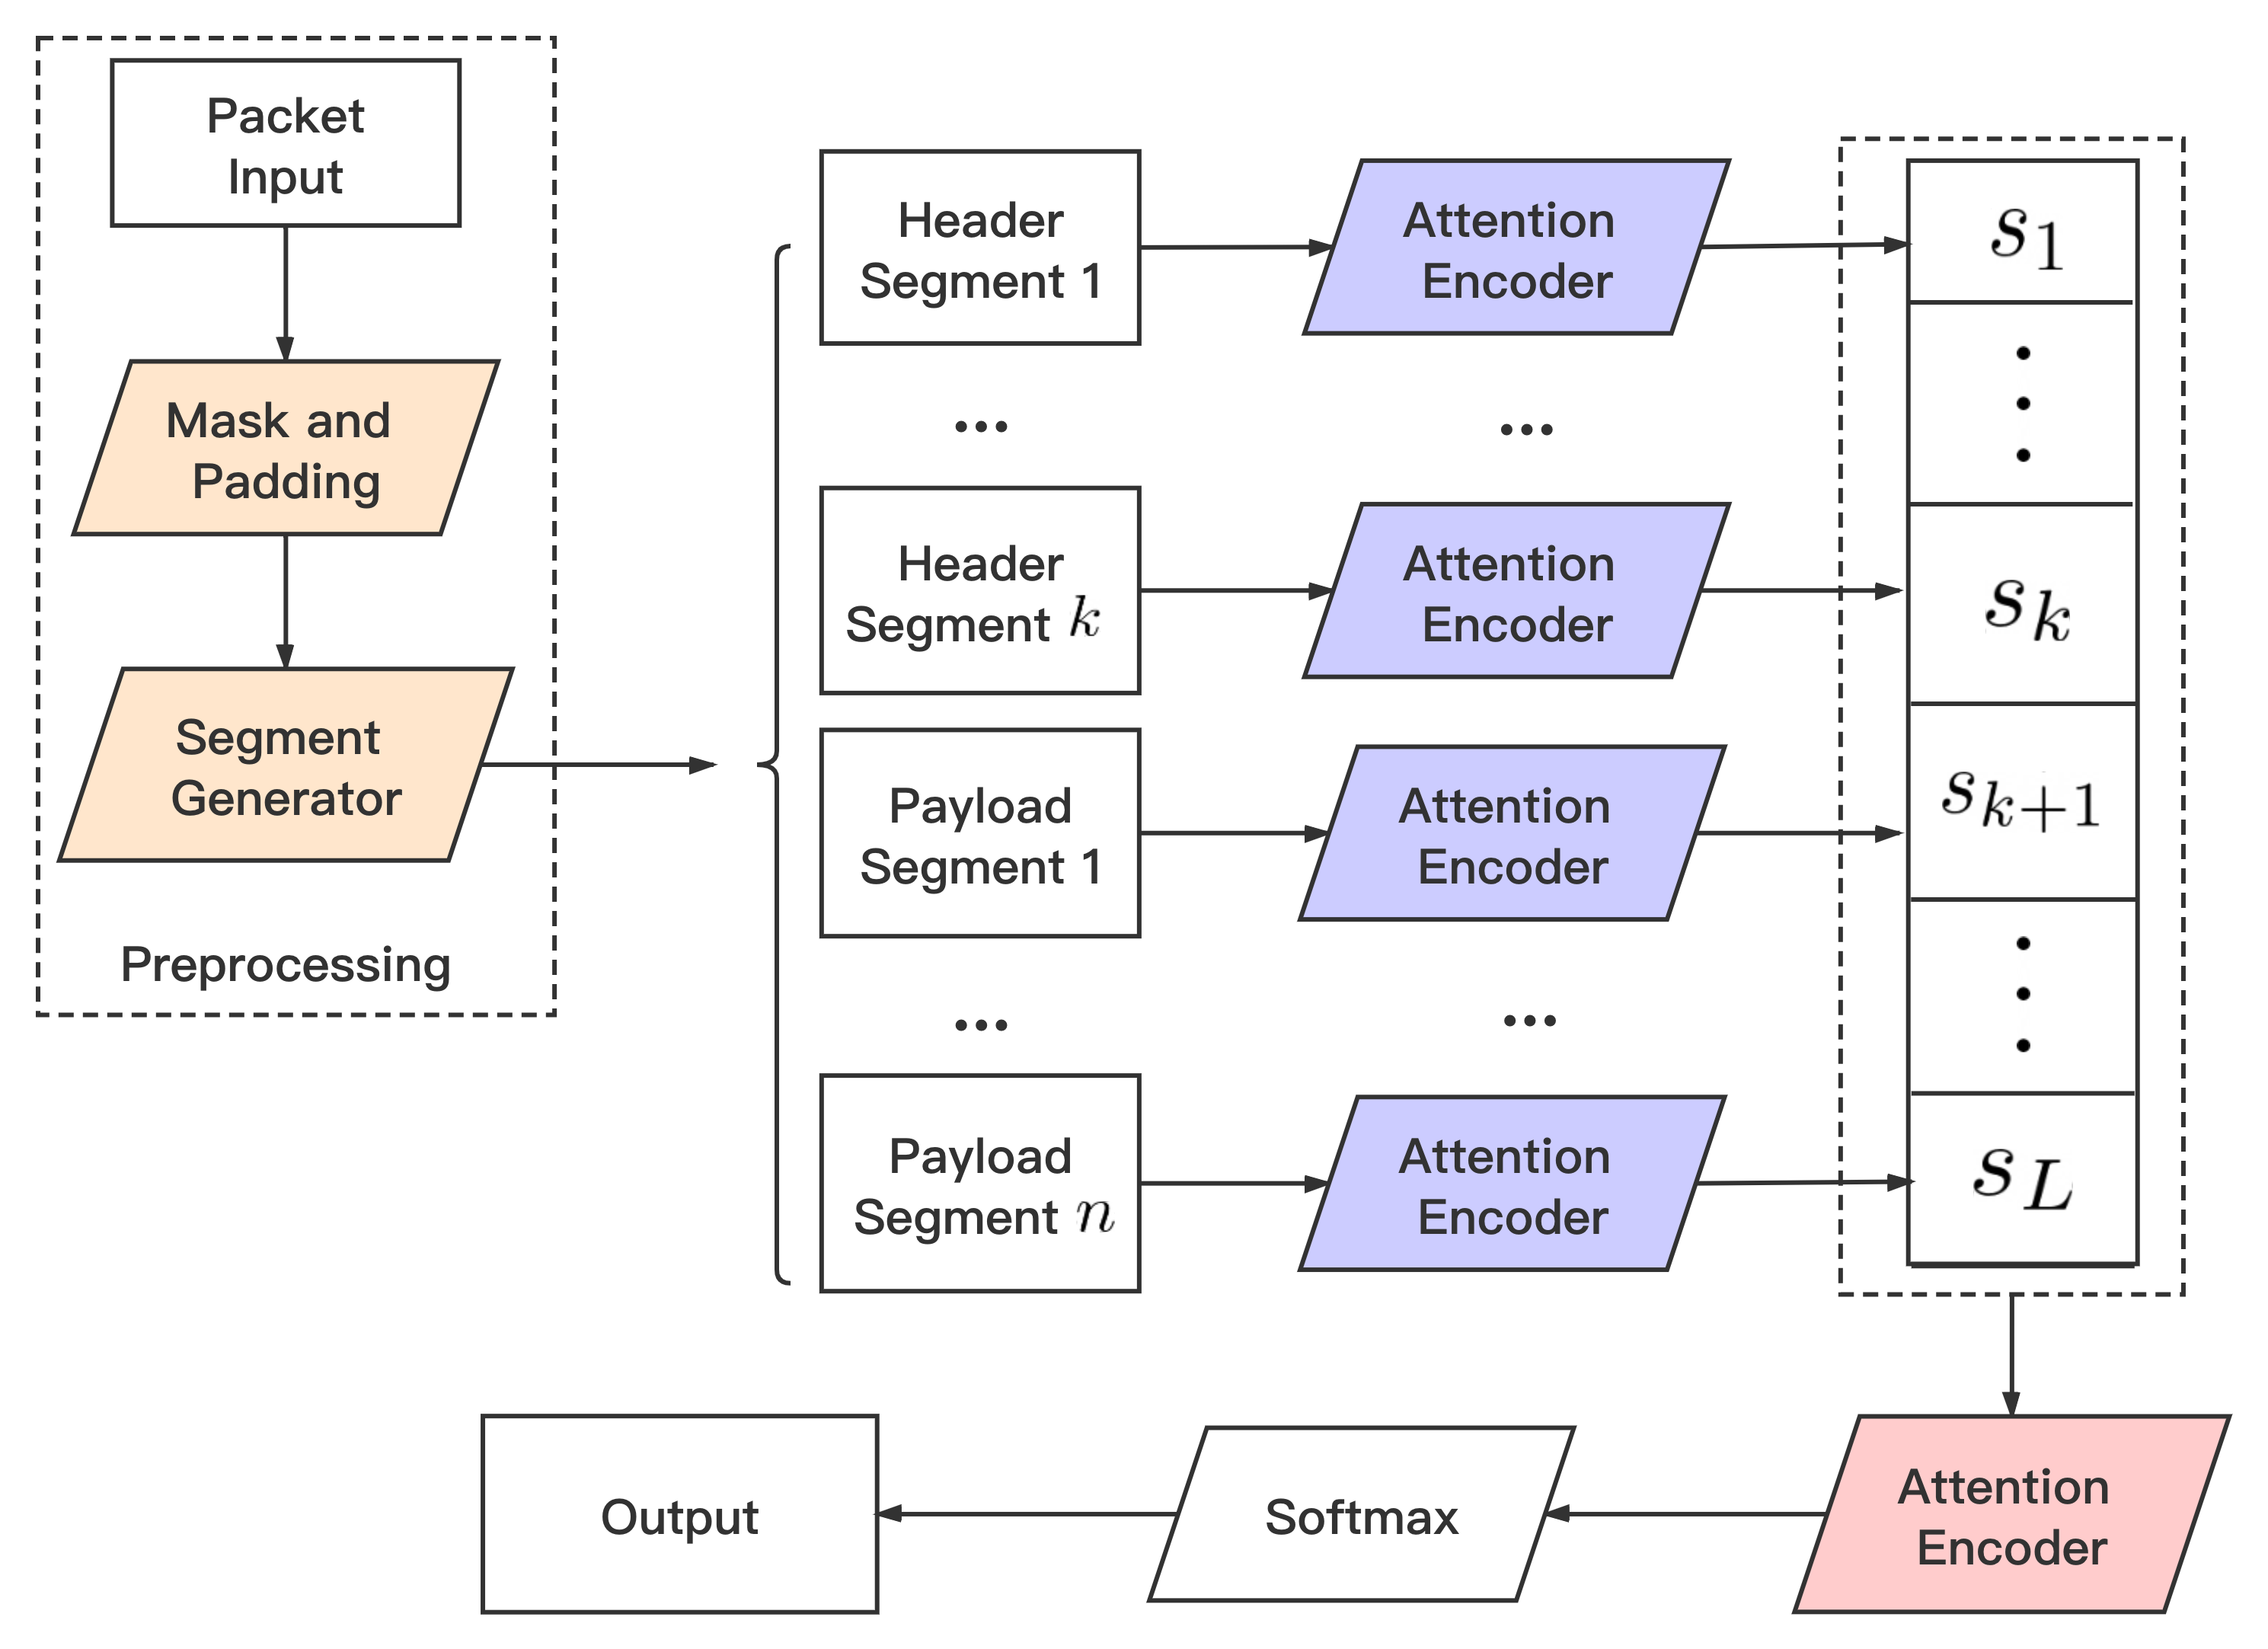
\includegraphics[width=9.5cm]{Overall_EBSNN.png}}
	\caption{EBSNN 整体架构}
	\label{fig1}
\end{figure}

在本节中,我们将详细介绍字节段神经网络(EBSNN)的架构。EBSNN的初始目标是将单个数据包划分为相应的应用或网站。EBSNN在数据包级的整体结构如图1所示。在我们的模型中,每一个单包都经过预处理后送入段生成器,并分解成一系列段,包括头段和有效载荷段。随后,注意力编码器将每个段转化为段向量。然后,将数据包的所有这些向量组合起来,放入另一个注意力编码器中,得到整个数据包的表示向量(在图~\ref{fig1}中,不同颜色的注意力编码器具有不同的RNN层)。最后,将表示向量引入softmax函数,计算出数据包的预测类。本方法的详细内容将在以下几个小节中描述。第~\ref{prep}小节介绍了预处理的细节,特别是分段生成器的细节;第~\ref{model}小节给出了所提出的模型的形式定义;第~\ref{flow}小节描述了我们所提出的模型在网络流级分类中的扩展。

\subsection{预处理}
\label{prep}

为了将原始数据转化为适合模型的合适表示方式,我们首先需要对原始数据包进行预处理。整个数据包在应用层上被分割成头文件和有效载荷。我们首先读取二进制格式的数据包,并将其呈现为一个范围为[0,255]的8位整数序列。然后,段生成器将该序列分解成固定长度N的字节段,称为段长。字节段有两种,即从头部产生的头部段和从有效载荷产生的有效载荷段。为了得到有效载荷段,在大多数情况下,有效载荷的字节总数不是段长的倍数 ,在有效载荷的末尾垫入0,字节构造一个段,因此段的数量为 $\lceil M / N \rceil$,其中M为有效载荷的长度。段生成器提供了原始有效载荷的简单表示。有效载荷段中的每个字节都可以看作是一个字符。因此,一个有效载荷段类似于自然语言中的一个句子,那么一个数据包就可以看作是一个文档。

\begin{figure}[!tp]
	\centerline{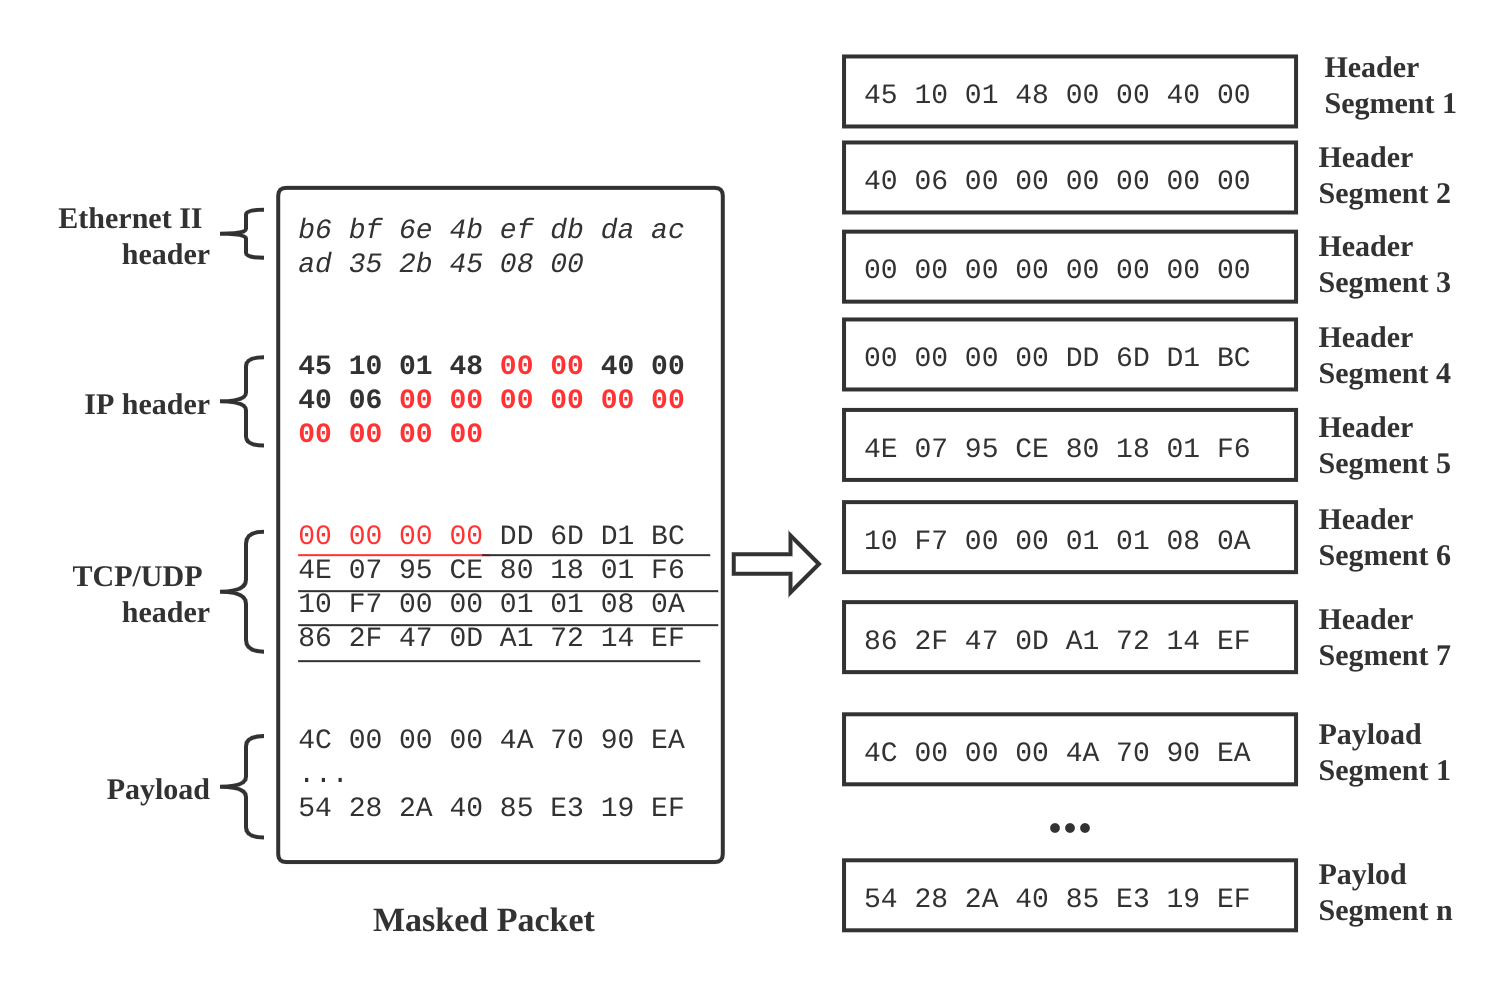
\includegraphics[width=10cm]{BSNN_Segment.png}}
	\caption{掩蔽后的包的段生成器实例}
	\label{fig2}
\end{figure}

与BSNN~\cite{bsnn}相比,我们在EBSNN中加入了包头的侧信道特征。除了有效载荷段外,我们还从包头中获取头段。数据包头由以太网II头、IP头和TCP/UDP头组成。虽然包头信息可以被利用来进行流量分类,但并不是所有的包头位都是有用的,部分包头位(如IP头中的源地址和目的IP地址)可能会导致过拟合。因此,我们首先对报头中的一些字段进行屏蔽,然后从报头中生成报头段。

\begin{enumerate}
	\item Ethernet II头: 由于该头只包含EtherType以及源地址和目的MAC地址,我们干脆放弃整个Ethernet II头。
	\item IP 头: 一些不提供有用信息的字段,如校验(checksum)和识别(identification)。另外,IP地址是个人数据。因此,我们做一些掩码工作,即把IP头中的一些字段用0代替:IP标识(IP头中的32$\sim$37位)、IP校验和(80$\sim$95位)、源IP地址(80$\sim$95位)、目的IP地址(96$\sim$127位)。之后,包括填充在内的段生成器与有效载荷段的段生成器相同。
	\item TCP/UDP 头: 与IP头类似,我们将源端口(0$\sim$15位)和目的端口(16$\sim$31位)用0代替。
\end{enumerate}

按照上述的方式,我们得到IP头段、TCP/UDP头段和有效载荷段。每一个段都是一个整数序列,在输入一个注意力编码器之前其长度为N。注意力编码器的目标是寻求数据包的最佳表示,并理解数据包。与手工制作的侧通道特征不同~\cite{moore2005discriminators},我们提出的EBSNN模型通过使用随机梯度下降优化器(如Adam~\cite{Adam})自动学习和选择比手工制作方法更合适的侧通道特征。

图~\ref{fig2}是段生成的一个例子。图中,左边部分是十六进制的屏蔽数据包,其中两个数字代表一个字节。图中斜体部分为以太网II头,在预处理时将其删除。数据包中粗体部分表示IP头,下划线部分表示TCP头。红色的零是数据包中被屏蔽的内容。在这个例子中,数据包被分成了N=8个短段(见图中右边部分),其中,一个段涉及8字节。在图中,有7个头段和n个有效载荷段。

\subsection{模型}
\label{model}

EBSNN通过采用分层RNN单元,结合每个字节和每个片段的上下文信息,实现对输入序列的合理表示。此外,它还使用关注层来找出哪部分对整个数据包是重要的。整个数据包的集合可以表示为 $A=\{\{a_{(i,n)} \}_{(n=1)}^N \}_{(i=1)}^L$,其中 $a_{(i,n)}$表示段i中的第n个字节 ,包括头段和有效载荷段,L是段的数量。为了将RNN单元应用到数据包中,我们需要将字节嵌入到向量中。如上所述,字节 $a_{(i,n)}$是介于0到255,之间的整数,可以将其转化为256维的独热向量。然后,将独热向量嵌入到稠密向量$x_{(i,n)}\ in \mathbb{R}^E$中。为了从片段中获取信息,我们采用了一个RNN结构,其注意力机制的灵感来自于HAN~\cite{b29}。这个结构在下文中被称为注意力编码器。起初,我们得到:
\begin{align}
	\begin{split}
		[h_{i,1}, \cdots, h_{i,N}] = \textsf{RNN}^{(1)}([x_{i,1}, \cdots, x_{i,N}]),
	\end{split}
\end{align}
其中 $\textsf{RNN}^{(1)}(\cdot)$ 表示隐藏大小为 $r$ 的RNN层(如LSTM或GRU)。相对于 $x_{i,n}$ 的注意力输出是$h_{i,n} \in \mathbb{R}^{f}$,其中$f$是$r$乘以RNN的方向数。注意力编码器中的RNN结构可以是单向的,也可以是双向的。

接下来,将一个网段中所有字节的输出,$h_{i,1}, \cdots, h_{i,N}$ 合并为一个段矩阵,$H_i  = [h_{i1}, \cdots, h_{iN}]^\top \in \mathbb{R}^{N \times f}$,以代表整个段。具体来说,由于不同的字节在流量分类中可能具有不同的重要性,因此采用关注机制对输出进行整合。

形式上,对于 $H_i$ 的注意力输出 $s_i \in \mathbb{R}^f$ 为:
\begin{align}
	\begin{split}
		s_i &= \text{Attention}(q, H_i) \\
		&\coloneqq H_i^\top \cdot \text{softmax}(\text{FC}(H_i) \cdot q),
	\end{split}
	\label{attention_encoder}
\end{align}
其中 $\text{FC}(\cdot)$ 表示全连接层:$\text{FC}(H_i) \coloneqq \tanh(H_i W_g + b_g) \in \mathbb{R}^{N \times f}$。在上式中,$q \in \mathbb{R}^{f \times 1}$ 是段中信息量最大的字节的抽象表示,它是随机初始化的。 将向量归一化为概率分布,其定义为:
\begin{equation}
	\text{softmax}(z)_i \coloneqq \frac{\exp{z_i}}{\sum_{j=1}^n \exp{z_j}},
\end{equation}
其中 $z \in \mathbb{R}^n$ 是未归一化的输入向量,输出也是一个 $n$ 维向量。

\begin{figure}[!tp]
	\centerline{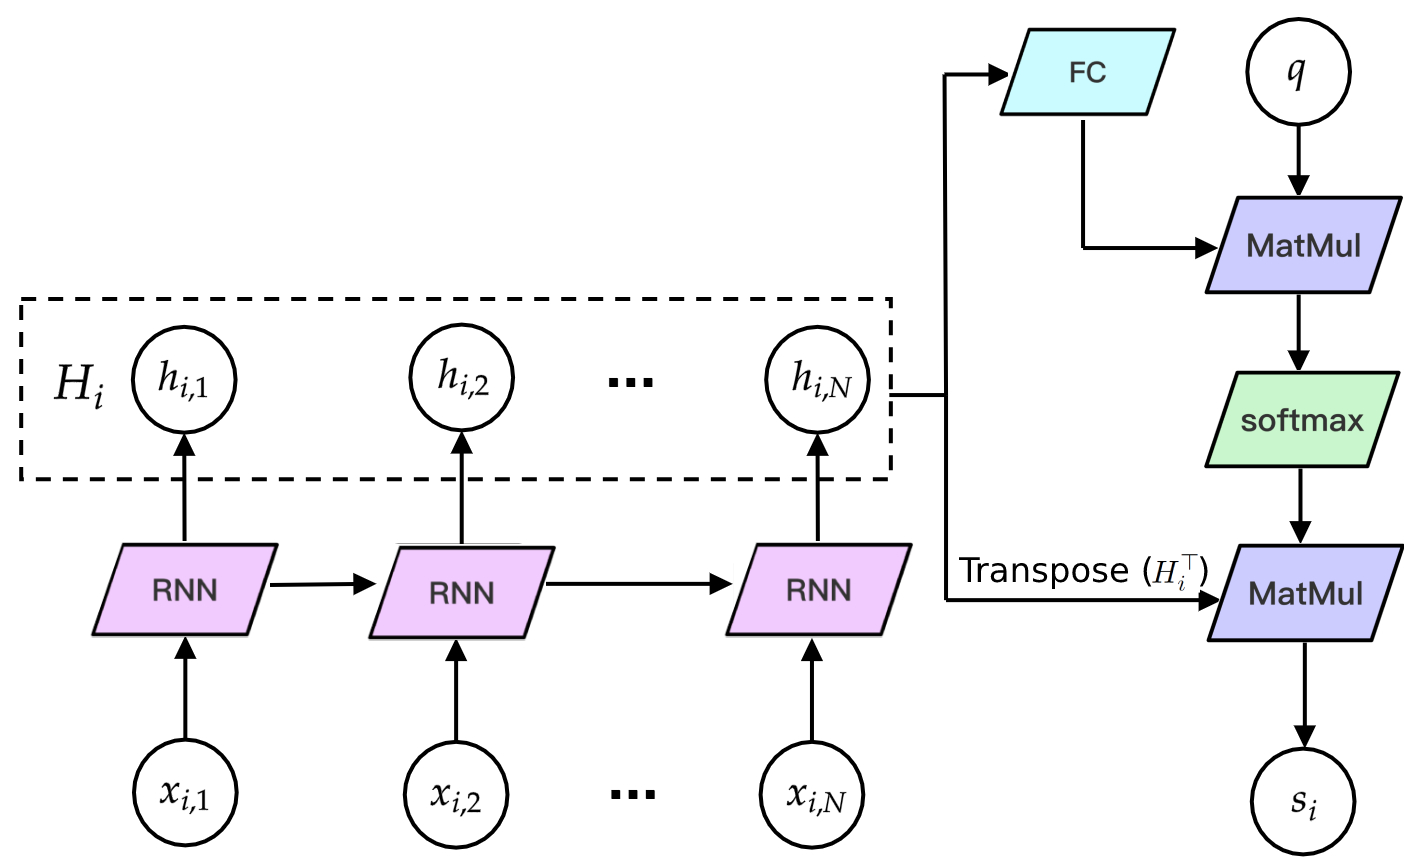
\includegraphics[width=9.0cm]{EBSNN_attention.png}}
	\caption{注意力编码器的结构}
	\label{fig_attention}
\end{figure}


从 $[x_{i,1}, \cdots, x_{i,N}]$ 到 $s_i$ 的变换称为注意力编码器:$s_i = \text{AttEncoder}([x_{i,1}, \cdots, x_{i,N}])$。图~\ref{fig_attention}为注意力编码器的整体结构,其中输入为 $[x_{i,1}, \cdots, x_{i,N}]$,输出为 $s_i$。图中MatMul表示矩阵乘法。使用相同的注意力编码器与相同的RNN层$\textsf{RNN}^{(1)}(\cdot)$ ,每个段都被转换为新的表示。我们将数据包的所有段的表示集合表示为 $S = [s_1, \cdots, s_L] \in \mathbb{R}^{f \times L}$。请注意,$S$是一系列的向量$[x_{i,1}, \cdots, x_{i,N}]$,就像一个单一的嵌入段。因此,我们采用另一个不同的$\textsf{RNN}^{(2)}(\cdot)$的注意力编码器来从 $S$ 得到整个包的注意力输出。最后,得到整个数据包的表示向量 $d = \text{AttEncoder}([s_1, \cdots, s_L]) \in \mathbb{R}^f$。由于我们已经有了数据包的表示 $d$,我们可以转向分类问题。对于 $C$ 分类,$d$ 可以将其转化为一个 $C$-维向量 $\tilde{y}= \text{softmax}(Wd+b)$,其中 $\tilde{y} \in \mathbb{R}^C$。因此,我们模型的整个过程可以表述为:
\begin{equation}
	\tilde{y} = \text{EBSNN}(A; \theta),
\end{equation}
其中 $\theta$ 为EBSNN的模型参数。

考虑到训练损失,我们在EBSNN中采用了焦点损失~\cite{8417976},因为它在不平衡多分类问题上表现出强大的优势。焦距损失的关键思想是,那些难以训练的实例对整个神经网络来说是重要的。对于 $C$-类分类的焦点损失可以简单计算如下:
\begin{equation}
	\text{FL}(y, \tilde{y}; \alpha, \beta) \coloneqq -\alpha(1 - \tilde{y}_l)^\gamma \log(\tilde{y}_l),
\end{equation}
其中 $y \in \mathbb{R}^C$ 是数据包的真实标签、$\alpha$ 是类权重和聚焦参数的独热向量。 $l$ 是真实标签,使得 $y_l = 1$ 和其他 $y_i \ (i \ne l)$ 都是零。$\tilde{y} \in \mathbb{R}^C$ 是我们提出的模型预测的标签的概率分布。

综上所述,EBSNN的迷你批量输入和参数为 $\mathcal{X}$ 和 $\theta$。在优化算法方面,我们采用Adam优化器~\cite{Adam}。

\subsection{扩展到网络流级分类}
\label{flow}

BSNN的初始目标是识别单个数据包,并在数据包级进行分类。在EBSNN中,我们对BSNN~\cite{bsnn}进行了扩展,通过引入聚合策略 $\text{agg}(\cdot): \mathbb{R}^{k \times C} \rightarrow \mathbb{R}^{C}$ 使其适合于流级分类。有研究~\cite{b12, MAAF}表明,流的前 $k$ 个数据包涉及流的重要信息。因此,流中第一个具有非空的应用级有效载荷的数据包可以代表流。与BSNN相比,EBSNN提供了流层面的支持,可以用来对整个流进行分类。

\begin{figure}[!tp]
	\centerline{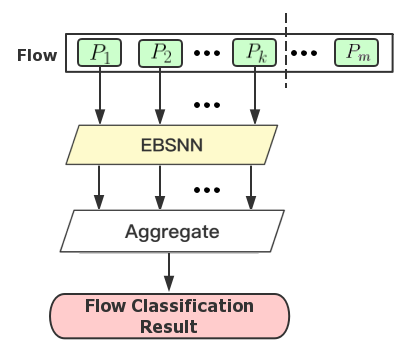
\includegraphics[width=7cm]{BSNN_Extension_Flow.png}}
	\caption{网络流级别分类扩展的工作流}
	\label{fig_extension_flow}
\end{figure}

正如我们在上一小节中提到的,EBSNN学习每个数据包的注意力编码表示d,并利用softmax函数计算数据包标签的概率分布 $\hat{y}$。图~\ref{fig_extension_flow}展示了扩展的整体工作流程和架构。一个流由一个数据包序列组成,包括一些零长度的数据包(如ACK和SYN)。让来自数据集的流为 $x = [P_1, P_2, \cdots, P_k, \cdots, P_m]$,其中$P_i$是流中第$i$-个具有非空的应用级有效载荷的数据包,它涉及头和有效载荷。由于流中的前几个数据包在网络流分类中起着至关重要的作用,我们只对流中具有非空应用级有效载荷的前k个数据包应用EBSNN。之后,可以得到这些数据包的 softmax 输出。最后,我们对这些输出进行聚合,得到流的标签。详细来说,这些聚合策略包括softmax输出和数据包结果的投票之和等。

值得一提的是,流量级分类方法~\cite{b12, MAAF}主要是基于特定的侧通道特征,如长度和方向。这些侧信道特征主要是从原始头(如TCP头)中提取的。除了常用的长度和方向特征外,数据包头还提供了更多的特征,如TCP头中的选项字段和TLS握手元数据。与这些方法相比,原始的数据包头被输入到EBSNN中,这样涉及到更多的侧信道特征(如TCP头中的选项字段的特征),我们的方法会自动学习最合适的侧信道特征。因此,EBSNN集中了头中的侧信道特征和有效载荷中的内容数据这两个方面更全面的信息。

\section{网络流量保护}

\begin{figure}[!tp]
	\centerline{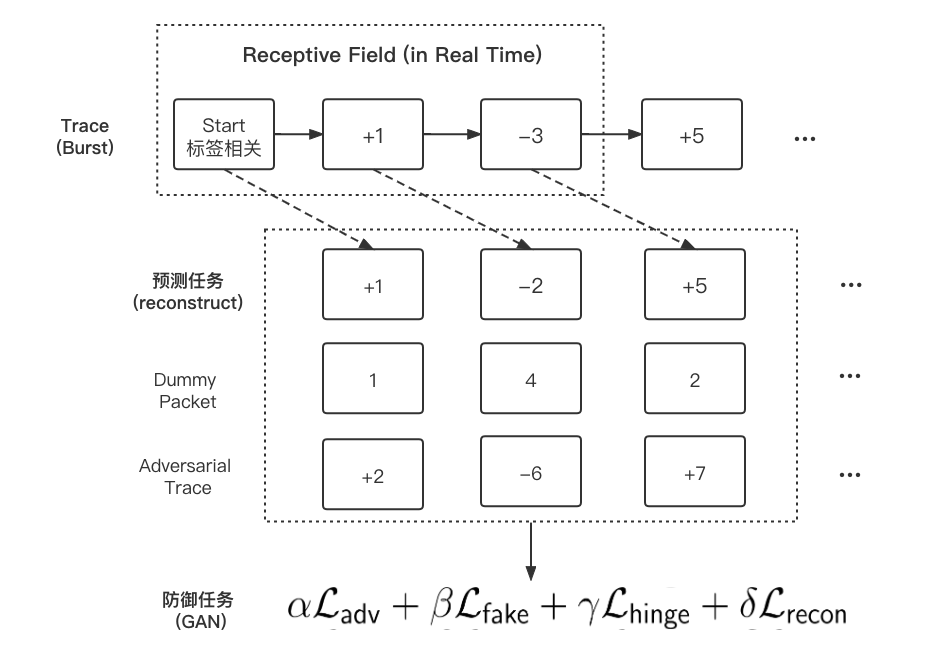
\includegraphics[width=12cm]{Practicable WF Defense.png}}
	\caption{网络流量保护工作原理}
	\label{fig:flow_defense}
\end{figure}

在本研究中,我们使用基于注意力机制的序列模型和生成式对抗网络(GAN)来自动的在网络流中插入噪声数据包,以使得攻击者无法通过网络流量分类方法进行攻击。
总体的工作原理如图~\ref{fig:flow_defense}所示。
模型主要分为生成器和判别器两个部分,生成器用于给定当前已发送出去的部分网络流量数据包的信息,计算得到下一次发送数据包的时候需要添加的噪声数据包的数量。
而判别器则是攻击者使用的一个网络流量分类模型,可以是白盒(攻击者使用的模型的具体架构和参数我们都知道)也可以是黑盒(我们无法获得攻击者使用的模型的具体信息)。
训练则是按照 GAN 训练的方式来进行:生成器和判别器轮流训练,通过精心设计的目标函数使得两个模块互相竞争,共同增强。

给定当前已经发送的包长序列 $\tilde{\boldsymbol{x}} = [x_1, \cdots, x_n]$,例如 $[+600, -1500, -120, +738, +289, -200, -400, -1400]$,正数代表正方向(实现规定好,例如客户端到服务端),负数代表负方向。
因为像洋葱网络之类的工具产生的流量的每个数据包的长度都一样,不失一般性地,我们首先根据每个包的方向将其映射到 $\{-1, +1\}^n$ 空间。
例如 $[+1, -1, -1, +1, +1, -1, -1, -1]$。
然后我们将其转化为突发序列 $\boldsymbol{x} \in \mathbb{Z}^n$,突发只指相同方向连续的数据包的累计个数(或大小)。
因为在实际网络设备中,为了提高效率,数据包的发送都会存入到一个队列中,当队列满才会发送这些数据包。
所以我们将其转化为突发序列有助于更加高效和符合实际地进行网络流量保护。
上述的例子转化为突发序列为 $[+1, -2, +2, -3]$。
攻击者可以训练出一个网络流量分类模型 $c = \text{argmax} \mathbb{F}_{\text{attack}} (\boldsymbol{x})$ 来对网络流量进行分析,并得到网络流量对应的网站、应用等类别标签 $c$,进而获取用户的隐私。

为了进行网络流量保护,我们将会在每一个突发中加入一些噪声数据包(对抗扰动),使得攻击者的攻击模型无法正常工作。
而这些对抗扰动的数量由防御模型计算得到,即噪声数据包序列 $\delta = \mathbb{F}_{\text{defense}}(\boldsymbol{x}) \in \mathbb{Z}^n$。
因为数据包突发序列是有方向的,而我们添加的噪声数据包也需要严格按照方向,故需要限制 $\forall \delta_i, \text{sign}(\delta_i) = \text{sign}(x_i)$。
保护后的网络流量的突发序列可以表示为 $\hat{\boldsymbol{x}} = \boldsymbol{x} + \boldsymbol{\delta}$。
网络流量保护的目标主要有三个:

\begin{enumerate}
	\item 添加噪声数据包后的网络流量使得攻击者的网络流量分析模型得到错误的标签结果,$\mathbb{F}_{\text{attack}}(\hat{\boldsymbol{x}}) \ne c, c = \mathbb{F}_{\text{attack}}(\boldsymbol{x})$。
	\item 因为添加噪声数据包会带来带宽的额外负担以及产生延迟,所以我们需要尽可能在使得攻击者模型出错的前提下噪声数据包的数量足够少:$\min \sum_{i=1}^n |\delta_i|$。
	\item 当保护模型计算第 $i$ 个突发需要添加的噪声数据包的时候,只能知道已发送或者已接收的历史数据包 $[x_1, \cdots, x_i]$ 的信息,而无法知晓未来还没有发送或接收的数据包 $[x_{i+1}, x_{i+2}, \cdots]$ 的信息。也就是说,$\delta_i = \mathbb{F}_{\text{defense}}([x_1, \cdots, x_i])$。
\end{enumerate}

为了达到上述目的,我们结合序列模型、生成式对抗网络、对抗样本设计了一组新颖的目标函数,如图~\ref{fig:flow_defense}所示。
同时,为了增强我们的保护模型对流量序列特征的上下文语义的感知能力,我们的保护模型的输出除了噪声数据包的数量之外,还需要预测下一个(未来的)突发的大小 $\delta_i, x_{i+1}^{\text{(pred)}} = \mathbb{F}_{\text{defense}}([x_1, \cdots, x_i])$,理想情况下 $x_{i+1}^{\text{(pred)}} = x_{i+1}$,目标函数为:
\begin{align}
	&\mathcal{L} = \alpha \mathcal{L}_{\text{adv}} + \beta \mathcal{L}_{\text{fake}} + \gamma \mathcal{L}_{\text{hinge}} + \sigma \mathcal{L}_{\text{recon}} \\
	&\mathcal{L}_{\text{adv}} = \mathbb{E}_{\hat{\boldsymbol{x}} \sim T^\prime} \text{ReLU} \left(\mathbb{F}_{\text{attack}} (\hat{\boldsymbol{x}})_c - \max_{t \ne c} \mathbb{F}_{\text{attack}} (\hat{\boldsymbol{x}})_i \right) \\
	&\mathcal{L}_{\text{fake}} = \mathbb{E}_{\hat{\boldsymbol{x}} \sim T^\prime} \log (\mathbb{D}(\hat{\boldsymbol{x}})) \\
	&\mathcal{L}_{\text{hinge}} = \lVert \boldsymbol{\delta} \rVert_1 \\
	&\mathcal{L}_{\text{recon}} = \frac{1}{n} \sum_{i=1}^n |x^{\text{(pred)}}_i - x_i|
\end{align}
其中 $\mathbb{D}$ 是判别器,是一个二分类器,用于判断 $\hat{\boldsymbol{x}}$ 为生成器添加噪声的网络流量(输出为 $\hat{\boldsymbol{x}}$ 被判别为生成器添加噪声后的网络流量的概率)。
\begin{align}
	\mathcal{L}_{\text{D}} &= \mathbb{E}_{\boldsymbol{x} \sim T} \log (\mathbb{D}(\boldsymbol{x})) + \mathbb{E}_{\hat{\boldsymbol{x}} \sim T^\prime} \log (\mathbb{D}(1 - \hat{\boldsymbol{x}}))
\end{align}

保护模型的网络结构定义为第~\ref{model}小节说述的注意力编码器 $\text{AttEncoder}(\cdot)$。

\chapter{现有工作基础}

\begin{itemize}
	\item \textbf{课程情况}:已完成培养计划里除专业实践、文献综述与选题报告外的所有课程。
	\item 已完成文献阅读与调研。
	\item \textbf{网络流量分类}:
	\begin{itemize}
		\item 实现提出的方法的代码。
		\item 收集网站识别任务的数据集,处理应用识别任务的数据集。
		\item 在两个数据集上进行充分的实验,对超参数和模型架构进行实验。
	\end{itemize}
	\item \textbf{网络流量保护}:
	\begin{itemize}
		\item 实验提出的方法的大部分代码。
		\item 初步实验结果。
	\end{itemize}
	\item \textbf{已接收论文成果}:
	\begin{itemize}
		\item (清华 A 类期刊学生一作)X. Xiao, W. Xiao, R. Li, X. Luo, H. -T. Zheng and S. -T. Xia, "EBSNN: Extended Byte Segment Neural Network for Network Traffic Classification," in IEEE Transactions on Dependable and Secure Computing, doi: 10.1109/TDSC.2021.3101311.
	\end{itemize}
\end{itemize}

\section{EBSNN 网络流量分类实验验证}

为了评估EBSNN的性能,我们在本节提供了大型新的真实世界数据集上的详细实验结果。首先,我们对数据集和指标进行了解释。然后,我们分析了我们模型的参数和网络结构的影响。此外,在数据包层面对应用识别任务进行了深入的实验,并详细介绍了与其他方法的比较。网站与应用不同,网站是互联网内容的另一种表现形式,其中包含了更多的噪声流量,因此,网站识别任务在数据包层面进行了彻底的实验,并与其他方法进行了详细的比较。因此,我们进行了网站识别任务,以验证EBSNN在该任务上对更多噪声数据的鲁棒性。此外,我们还进行了大量的流量层面的应用识别实验。所有的实验都是在128GB内存、Intel Xeon Silver 4210 CPU、NVIDIA 2080Ti GPU的服务器上进行的。

\subsection{数据集}

在实验中,使用D1和D2两个数据集,分别用于应用识别和网站识别两个不同的任务。D1是一个大型的真实世界的应用识别数据集,由29种流行的应用组成。我们的数据集中出现了很多有代表性的应用,包括电子邮件、音乐、视频、社交网络、搜索和购物等。在实际的网络环境中,通过追踪相应的应用进程来捕获特定协议的数据报。具体来说,流量采集器首先获取目标应用的套接字信息,然后对数据包进行过滤,将数据包在真实的网络环境中进行相应的追踪。然后,根据套接字信息对数据报进行过滤和保存。通过这种方式,可以无噪音地收集网络流量。需要注意的是,我们的数据集包括加密和未加密的网络流量数据,这反映了真实的网络环境。每个应用中数据包数量的详细信息可以在表~\ref{tab1}中找到。从统计信息中可以看出,数据集中各个类的数据包数量差异较大,即类不平衡。这样的类不平衡现象在实际网络场景中经常出现。


\begin{table}[!tp]
	\scriptsize
	\caption{用应用识别任务的数据集 \textbf{D1} 的详情}
	\begin{center}
		\begin{tabular}{c|c|c||c|c|c}
			\noalign{\hrule height 1pt}
			\textbf{ID} &\textbf{应用}& \#\textbf{数据包数量} & \textbf{ID} &\textbf{应用}& \#\textbf{数据包数量}\\
			\noalign{\hrule height 1pt}
			1 & Vimeo & $35267$ & 16 & iTunes & $18066$ \\ \hline
			2 & Spotify & $10034$ & 17 & Twitter & $9314$ \\ \hline 
			3 & VoipBuster & $360403$ & 18 & JD & $19487$ \\ \hline
			4 & Sina UC & $155951$ & 19 & SOHU & $39014$ \\ \hline 
			5 & Netease Cloud Music & $84873$ & 20 & Youtube & $40856$ \\ \hline
			6 & Sina Weibo & $49796$ & 21 & Youku & $99909$ \\ \hline
			7 & Baidu & $36364$ & 22 & Netflix & $55189$ \\ \hline
			8 & Tudou & $89720$ & 23 & AIM Chat & $17260$ \\ \hline 
			9 & Amazon & $14530$ & 24 & Kugou & $170167$ \\ \hline
			10 & Thunder & $64325$ & 25 & Skype & $632501$ \\ \hline 
			11 & Gmail & $11004$ & 26 & Facebook & $245434$ \\ \hline
			12 & PPLive & $181113$ & 27 & Google & $6767$ \\ \hline
			13 & QQ & $14045$ & 28 & MS-SQL & $20882$ \\ \hline
			14 & Taobao & $31136$ & 29 & MS-Exchange & $1720$ \\ \hline
			15 & Yahoo Mail & $38948$ & - & Average & $88071$ \\
			\noalign{\hrule height 1pt}
		\end{tabular}
		\label{tab1}
	\end{center}
\end{table}

络场景中经常出现 。
另一方面,D2是另一个用于网站识别的大型真实世界数据集,包含20种热门网站。我们在2020年通过在隔离环境中运行定制的轻量级浏览器和网络流量转储工具(即WireShark)来收集D2。隔离环境是用Docker和网络命名空间构建的,其中只运行浏览器和WireShark。为了尽可能多地收集纯网络流量,自定义浏览器禁用了所有嘈杂的网络流量(如搜索推荐、浏览器更新检查和账户同步)。对于一些必须登录账号的网站,如QQ邮箱、微博等,我们手动登录个人账号来获取真实的网络流量。与应用识别相比,网站识别是一项噪音较多的任务,很多网站共享存储在同一个CDN的静态文件,表现出相似的行为。具体来说,D2由网站组成。JD、网易云音乐、TED、亚马逊、百度、必应、豆瓣、Facebook、谷歌、IMDb、Instagram、爱奇艺、QQ邮箱、Reddit、淘宝、铁霸、Twitter、新浪微博、优酷、Youtube。这些网站几乎涵盖了日常生活的方方面面。大部分流量采用https作为传输协议。因此,https中的数据都是加密的,无法通过目的IP和端口进行区分。统计信息如表~\ref{tab_websites}所示。

\begin{table}[!tp]
	\scriptsize
	\caption{用于网站识别任务的数据集 \textbf{D2} 的详情}
	\begin{center}
		\begin{tabular}{c|c|c||c|c|c}
			\noalign{\hrule height 1pt}
			\textbf{ID} &\textbf{网站}& \#\textbf{数据包数量} & \textbf{ID} &\textbf{网站}& \#\textbf{数据包数量}\\
			\noalign{\hrule height 1pt}
			1 & JD & $150,157$ & 11 & Instagram & $123,930$ \\ \hline
			2 & Netease Cloud Music & $152,988$ & 12 & iQIYI & $193,280$ \\ \hline
			3 & TED & $262,622$ & 13 & QQ Mail & $97,661$ \\ \hline
			4 & Amazon & $145,377$ & 14 & Reddit & $230,603$ \\ \hline
			5 & Baidu & $137,859$ & 15 & Taobao & $227,034$ \\ \hline
			6 & Bing & $161,689$ & 16 & Tieba & $125,235$ \\ \hline
			7 & Douban & $138,904$ & 17 & Twitter & $229,780$ \\ \hline
			8 & Facebook & $249,179$ & 18 & Sina Weibo & $323,014$ \\ \hline
			9 & Google & $69,251$ & 19 & Youku & $137,877$ \\ \hline
			10 & IMDb & $253,404$ & 20 & Youtube & $315,101$ \\
			\noalign{\hrule height 1pt}
		\end{tabular}
		\label{tab_websites}
	\end{center}
\end{table}

\subsection{网络包级别应用识别任务}


\begin{table*}[!htp]
	\tiny
%	\caption{数据集 \textbf{D1} 上的网络包级别应用识别任务实验结果}
	\begin{center}
%		\begin{sideways}
		\begin{tabular}{c|c|c c c|c c c|c c c|c c c}
			\noalign{\hrule height 1pt}
			\multirow{2}{*}{\textbf{ID}} & \multirow{2}{*}{\textbf{Application}} & \multicolumn{3}{c}{\textbf{Securitas-C4.5}} &\multicolumn{3}{c}{\textbf{Securitas-SVM}}& \multicolumn{3}{c}{\textbf{Securitas-Bayes}} &\multicolumn{3}{c}{\textbf{DP-SAE}}  \\
			\cline{3-14}
			& & $R.$ & $P.$ & $F_1.$ & $R.$ & $P.$ & $F_1.$ & $R.$ & $P.$ & $F_1.$ & $R.$ & $P.$ & $F_1.$ \\ 
			\noalign{\hrule height 1pt}
			1 & Vimeo & $0.9801$ & $0.9875$ & $0.9838$ & $0.9167$ & $0.9625$ & $0.9390$ & $0.9106$ & $0.9675$ & $0.9382$ & $0.9133$ & $0.9562$ & $0.9343$ \\\hline
			2 & Spotify & $0.9556$ & $0.9675$ & $0.9615$ & $0.8990$ & $0.8675$ & $0.8830$ & $0.8990$ & $0.8900$ & $0.8945$ & $0.7682$ & $0.7643$ & $0.7662$ \\\hline
			3 & VoipBuster & $0.7813$ & $0.9825$ & $0.8704$ & $0.5783$ & $0.9975$ & $0.7321$ & $0.7007$ & $0.9950$ & $0.8223$ & $0.9908$ & $0.9931$ & $0.9920$ \\\hline
			4 & Sina UC & $0.9807$ & $0.8875$ & $0.9318$ & $0.9398$ & $0.8200$ & $0.8758$ & $0.9368$ & $0.8525$ & $0.8927$ & $0.9747$ & $0.9945$ & $0.9845$ \\\hline
			5 & Netease Cloud Music & $0.9490$ & $0.9300$ & $0.9394$ & $0.9968$ & $0.7750$ & $0.8720$ & $0.9742$ & $0.8500$ & $0.9079$ & $0.7252$ & $0.9361$ & $0.8173$ \\\hline
			6 & Sina Weibo & $0.7073$ & $0.9425$ & $0.8081$ & $0.6365$ & $0.9675$ & $0.7679$ & $0.6812$ & $0.9350$ & $0.7882$ & $0.6595$ & $0.8009$ & $0.7233$ \\\hline
			7 & Baidu & $0.6913$ & $0.9350$ & $0.7949$ & $0.6770$ & $0.9325$ & $0.7844$ & $0.6893$ & $0.8875$ & $0.7760$ & $0.6166$ & $0.5921$ & $0.6041$  \\\hline
			8 & Tudou & $0.7255$ & $0.9450$ & $0.8208$ & $0.9427$ & $0.5350$ & $0.6826$ & $0.8960$ & $0.5600$ & $0.6892$ & $0.8518$ & $0.8060$ & $0.8282$  \\\hline
			9 & Amazon & $0.6893$ & $0.9375$ & $0.7945$ & $0.6437$ & $0.9350$ & $0.7625$ & $0.6692$ & $0.8800$ & $0.7603$ & $0.6489$ & $0.1889$ & $0.2926$  \\\hline
			10 & Thunder & $0.7451$ & $0.9575$ & $0.8381$ & $0.8379$ & $0.6075$ & $0.7043$ & $0.7922$ & $0.6575$ & $0.7186$ & $0.7880$ & $0.7755$ & $0.7817$  \\\hline
			11 & Gmail & $0.9281$ & $0.6450$ & $0.7611$ & $0.8621$ & $0.5000$ & $0.6329$ & $0.8258$ & $0.5450$ & $0.6566$ & $0.5475$ & $0.1808$ & $0.2719$  \\\hline
			12 & PPLive & $0.9529$ & $0.9100$ & $0.9309$ & $0.9969$ & $0.8000$ & $0.8877$ & $0.9971$ & $0.8625$ & $0.9249$ & $0.9619$ & $0.9354$ & $0.9485$  \\\hline
			13 & QQ & $0.9016$ & $0.6875$ & $0.7801$ & $0.8773$ & $0.5900$ & $0.7055$ & $0.8796$ & $0.6025$ & $0.7151$ & $0.7227$ & $0.3535$ & $0.4748$  \\\hline
			14 & Taobao & $0.7034$ & $0.9250$ & $0.7991$ & $0.6443$ & $0.9600$ & $0.7711$ & $0.6888$ & $0.9350$ & $0.7932$ & $0.7014$ & $0.7132$ & $0.7072$  \\\hline
			15 & YahooMail & $0.7490$ & $0.9400$ & $0.8337$ & $0.6736$ & $0.9650$ & $0.7934$ & $0.6878$ & $0.9475$ & $0.7971$ & $0.8619$ & $0.9241$ & $0.8920$ \\\hline
			16 & iTunes & $0.7058$ & $0.9475$ & $0.8090$ & $0.6594$ & $0.9775$ & $0.7875$ & $0.6797$ & $0.9550$ & $0.7942$ & $0.6395$ & $0.3501$ & $0.4525$  \\\hline
			17 & Twitter & $0.9705$ & $0.9875$ & $0.9789$ & $0.9459$ & $0.9175$ & $0.9315$ & $0.9397$ & $0.9350$ & $0.9373$ & $0.6448$ & $0.8486$ & $0.7328$  \\\hline
			18 & JD & $0.6861$ & $0.9125$ & $0.7833$ & $0.6562$ & $0.9400$ & $0.7729$ & $0.6904$ & $0.8975$ & $0.7804$ & $0.5623$ & $0.1737$ & $0.2654$  \\\hline
			19 & Sohu & $0.7050$ & $0.9200$ & $0.7983$ & $0.8922$ & $0.4550$ & $0.6026$ & $0.8683$ & $0.5275$ & $0.6563$ & $0.8483$ & $0.8531$ & $0.8507$  \\\hline
			20 & Youtube & $0.9777$ & $0.9850$ & $0.9813$ & $0.9442$ & $0.9300$ & $0.9370$ & $0.9398$ & $0.9375$ & $0.9387$ & $0.9416$ & $0.9293$ & $0.9354$  \\\hline
			21 & Youku & $0.9079$ & $0.7150$ & $0.8000$ & $0.9261$ & $0.5950$ & $0.7245$ & $0.8958$ & $0.6450$ & $0.7500$ & $0.8315$ & $0.8916$ & $0.8605$  \\\hline
			22 & Netflix & $0.9725$ & $0.9725$ & $0.9725$ & $0.9530$ & $0.8625$ & $0.9055$ & $0.9251$ & $0.9575$ & $0.9410$ & $0.9667$ & $0.9776$ & $0.9721$  \\\hline
			23 & Aimchat & $0.7446$ & $0.9550$ & $0.8368$ & $0.9696$ & $0.5575$ & $0.7079$ & $0.9405$ & $0.5925$ & $0.7270$ & $0.7118$ & $0.5379$ & $0.6128$  \\\hline
			24 & Kugou & $0.9860$ & $0.8775$ & $0.9286$ & $\textbf{1.0000}$ & $0.8225$ & $0.9026$ & $0.9941$ & $0.8425$ & $0.9120$ & $0.9926$ & $0.9602$ & $0.9761$  \\\hline
			25 & Skype & $0.7538$ & $0.9800$ & $0.8522$ & $0.9157$ & $0.1900$ & $0.3147$ & $0.7180$ & $0.9675$ & $0.8243$ & $0.9534$ & $0.9743$ & $0.9637$  \\\hline
			26 & Facebook & $0.9975$ & $0.9875$ & $0.9925$ & $0.9921$ & $0.9375$ & $0.9640$ & $0.9874$ & $0.9800$ & $0.9837$ & $0.9762$ & $0.9911$ & $0.9836$  \\\hline
			27 & Google & $0.9850$ & $0.9825$ & $0.9837$ & $0.9475$ & $0.9475$ & $0.9475$ & $0.9478$ & $0.9525$ & $0.9501$ & $0.6290$ & $0.3659$ & $0.4626$  \\\hline
			28 & MS-SQL & $0.9900$ & $0.9950$ & $0.9925$ & $0.9924$ & $0.9775$ & $0.9849$ & $0.9949$ & $0.9775$ & $0.9861$ & $0.9594$ & $0.9447$ & $0.9520$  \\\hline
			29 & MS-Exchange & $0.9813$ & $0.7645$ & $0.8595$ & $0.9881$ & $0.7238$ & $0.8356$ & $0.9806$ & $0.7355$ & $0.8405$ & $0.8342$ & $0.4826$ & $0.6114$  \\
			\noalign{\hrule height 1pt}
			- & Average & $0.8553$ & $0.9159$ & $0.8765$ & $0.8588$ & $0.7948$ & $0.7970$ & $0.8528$ & $0.8369$ & $0.8309$ & $0.8008$ & $0.7309$ & $0.7466$  \\\hline
			- & $Accuracy$ & \multicolumn{3}{c}{0.8674} & \multicolumn{3}{c}{0.8082} & \multicolumn{3}{c}{0.8325} & \multicolumn{3}{c}{0.9169} \\
			\noalign{\hrule height 1pt}
		\end{tabular}
%		\end{sideways}
	\begin{center}
		\begin{tabular}{c|c|c c c|c c c|c c c}
			\noalign{\hrule height 1pt}
			\multirow{2}{*}{\textbf{ID}} & \multirow{2}{*}{\textbf{Application}} & \multicolumn{3}{c}{\textbf{DP-CNN}} &\multicolumn{3}{c}{\textbf{EBSNN-GRU}}& \multicolumn{3}{c}{\textbf{EBSNN-LSTM}} \\
			\cline{3-11}
			& & $R.$ & $P.$ & $F_1.$ & $R.$ & $P.$ & $F_1.$ & $R.$ & $P.$ & $F_1.$ \\
			\noalign{\hrule height 1pt}
			1 & Vimeo & $0.9743$ & $0.9820$ & $0.9781$ & $0.9959$ & $0.9967$ & $0.9963$ & $\textbf{0.9984}$ & $\textbf{0.9991}$ & $\textbf{0.9988}$ \\\hline
			2 & Spotify & $0.9511$ & $0.9108$ & $0.9305$ & $0.9776$ & $0.9771$ & $0.9773$ & $\textbf{0.9935}$ & $\textbf{0.9915}$ & $\textbf{0.9925}$ \\\hline
			3 & VoipBuster & $0.9994$ & $0.9974$ & $0.9984$ & $0.9981$ & $\textbf{0.9998}$ & $0.9989$ & $\textbf{0.9991}$ & $\textbf{0.9998}$ & $\textbf{0.9995}$ \\\hline
			4 & SinaUC & $0.9998$ & $0.9992$ & $0.9995$ & $0.9999$ & $0.9999$ & $0.9999$ & $\textbf{1.0000}$ & $\textbf{1.0000}$ & $\textbf{1.0000}$ \\\hline
			5 & Netease Cloud Music & $0.9785$ & $0.9928$ & $0.9856$ & $0.9985$ & $0.9994$ & $0.9990$ & $\textbf{0.9999}$ & $\textbf{0.9997}$ & $\textbf{0.9998}$ \\\hline
			6 & Sina Weibo & $0.9519$ & $0.9796$ & $0.9656$ & $0.9994$ & $0.9969$ & $0.9981$ & $\textbf{1.0000}$ & $\textbf{0.9998}$ & $\textbf{0.9999}$ \\\hline
			7 & Baidu & $0.9227$ & $0.9284$ & $0.9255$ & $0.9865$ & $\textbf{0.9993}$ & $0.9929$ & $\textbf{0.9999}$ & $0.9985$ & $\textbf{0.9992}$ \\\hline
			8 & Tudou & $0.9880$ & $0.9899$ & $0.9890$ & $0.9985$ & $0.9992$ & $0.9989$ & $\textbf{0.9996}$ & $\textbf{0.9998}$ & $\textbf{0.9997}$ \\\hline
			9 & Amazon & $0.9250$ & $0.8737$ & $0.8986$ & $0.9993$ & $\textbf{1.0000}$ & $0.9997$ & $\textbf{1.0000}$ & $\textbf{1.0000}$ & $\textbf{1.0000}$ \\\hline
			10 & Thunder & $0.9737$ & $0.9955$ & $0.9845$ & $0.9990$ & $0.9973$ & $0.9981$ & $\textbf{0.9994}$ & $\textbf{0.9997}$ & $\textbf{0.9995}$ \\\hline
			11 & Gmail & $0.8653$ & $0.9109$ & $0.8876$ & $0.9886$ & $0.9523$ & $0.9701$ & $\textbf{0.9900}$ & $\textbf{0.9945}$ & $\textbf{0.9923}$ \\\hline
			12 & PPLive & $0.9932$ & $0.9829$ & $0.9880$ & $\textbf{0.9999}$ & $0.9972$ & $0.9985$ & $0.9998$ & $\textbf{0.9999}$ & $\textbf{0.9999}$ \\\hline
			13 & QQ & $0.9535$ & $0.9203$ & $0.9366$ & $0.9897$ & $0.9918$ & $0.9907$ & $\textbf{0.9982}$ & $\textbf{0.9975}$ & $\textbf{0.9979}$ \\\hline
			14 & Taobao & $0.9486$ & $0.9107$ & $0.9293$ & $0.9992$ & $0.9994$ & $0.9993$ & $\textbf{0.9997}$ & $\textbf{0.9997}$ & $\textbf{0.9997}$ \\\hline
			15 & YahooMail & $0.9958$ & $0.9854$ & $0.9906$ & $0.9994$ & $0.9992$ & $0.9993$ & $\textbf{1.0000}$ & $\textbf{1.0000}$ & $\textbf{1.0000}$ \\\hline
			16 & iTunes & $0.9529$ & $0.9125$ & $0.9323$ & $0.9914$ & $0.9975$ & $0.9944$ & $\textbf{0.9994}$ & $\textbf{1.0000}$ & $\textbf{0.9997}$ \\\hline
			17 & Twitter & $0.9726$ & $0.9898$ & $0.9811$ & $\textbf{0.9995}$ & $0.9989$ & $0.9992$ & $\textbf{0.9995}$ & $\textbf{1.0000}$ & $\textbf{0.9997}$ \\\hline
			18 & JD & $0.8763$ & $0.9251$ & $0.9000$ & $0.9985$ & $0.9990$ & $0.9987$ & $\textbf{0.9992}$ & $\textbf{0.9997}$ & $\textbf{0.9995}$ \\\hline
			19 & Sohu & $0.9795$ & $0.9759$ & $0.9777$ & $0.9974$ & $0.9911$ & $0.9942$ & $\textbf{0.9999}$ & $\textbf{0.9986}$ & $\textbf{0.9992}$ \\\hline
			20 & Youtube & $0.9806$ & $0.9794$ & $0.9800$ & $0.9930$ & $0.9969$ & $0.9950$ & $\textbf{0.9980}$ & $\textbf{0.9978}$ & $\textbf{0.9979}$ \\\hline
			21 & Youku & $0.9863$ & $0.9873$ & $0.9868$ & $0.9990$ & $0.9982$ & $0.9986$ & $\textbf{0.9995}$ & $\textbf{0.9999}$ & $\textbf{0.9997}$ \\\hline
			22 & Netflix & $0.9958$ & $0.9922$ & $0.9940$ & $0.9989$ & $0.9982$ & $0.9985$ & $\textbf{0.9994}$ & $\textbf{0.9991}$ & $\textbf{0.9992}$ \\\hline
			23 & Aimchat & $0.9206$ & $0.9299$ & $0.9252$ & $0.9606$ & $\textbf{0.9967}$ & $0.9783$ & $\textbf{0.9945}$ & $0.9962$ & $\textbf{0.9954}$ \\\hline
			24 & Kugou & $0.9982$ & $0.9942$ & $0.9962$ & $0.9996$ & $0.9996$ & $0.9996$ & $0.9999$ & $\textbf{0.9999}$ & $\textbf{0.9999}$ \\\hline
			25 & Skype & $0.9965$ & $0.9983$ & $0.9974$ & $0.9997$ & $0.9985$ & $0.9991$ & $\textbf{0.9998}$ & $\textbf{0.9993}$ & $\textbf{0.9996}$ \\\hline
			26 & Facebook & $0.9994$ & $0.9996$ & $0.9995$ & $0.9998$ & $0.9999$ & $0.9999$ & $\textbf{0.9999}$ & $\textbf{1.0000}$ & $\textbf{1.0000}$ \\\hline
			27 & Google & $0.9856$ & $0.9608$ & $0.9731$ & $\textbf{0.9978}$ & $\textbf{1.0000}$ & $\textbf{0.9989}$ & $\textbf{0.9978}$ & $\textbf{1.0000}$ & $\textbf{0.9989}$ \\\hline
			28 & MS-SQL & $0.9947$ & $0.9966$ & $0.9957$ & $0.9990$ & $0.9995$ & $0.9993$ & $\textbf{1.0000}$ & $\textbf{1.0000}$ & $\textbf{1.0000}$ \\\hline
			29 & MS-Exchange & $0.9788$ & $0.9390$ & $0.9585$ & $\textbf{0.9971}$ & $0.9971$ & $0.9971$ & $\textbf{0.9971}$ & $\textbf{1.0000}$ & $\textbf{0.9985}$ \\
			\noalign{\hrule height 1pt}
			- & Average & $0.9668$ & $0.9635$ & $0.9650$ & $0.9952$ & $0.9957$ & $0.9954$ & $\textbf{0.9987}$ & $\textbf{0.9990}$ & $\textbf{0.9988}$ \\\hline
			- & $Accuracy$ & \multicolumn{3}{c}{0.9887} & \multicolumn{3}{c}{0.9990} & \multicolumn{3}{c}{\textbf{0.9996}} \\
			\noalign{\hrule height 1pt}
		\end{tabular}
	\end{center}
	\label{tab2}
	\end{center}
\end{table*}


在本节中,我们重点关注多类应用识别任务。我们在这部分提供了EBSNN的详细结果,并与现有的方法~\cite{deep_packet,b25}进行了比较。Securitas是传统的机器学习方法,它在2016年被提出,并成为流量分类领域的最佳解决方案之一。另一方面,DeepPacket是典型的基于深度学习的方法。这两种方法和EBSNN都是在数据包层面识别网络流量,即可以识别一个单一数据包的应用。
Securitas是一种有效载荷级的流量分类方法。它使用LDA主题模型来提取特定应用的特征,然后再将这些特征分别反馈给传统的监督机器学习方法,如SVM、C4.5决策树和贝叶斯网络。Securitas是传统机器学习的经典流量分类方法,它致力于寻找合适的特征来构建机器学习分类器。
DeepPacket利用数据包中的有效载荷内容作为深度学习模型的输入,包括多层感知器、一维CNN和堆栈式自动编码器。作为一个利用深度学习从数据包中自动学习有用表示的框架,DeepPacket开启了在网络流量的分类任务中利用深度学习模型的趋势。

实验结果如上表所示,其中最好的是粗体字。指标 R., P. 和 $F_1$ 分别代表 Recall, Precision, 和 $F_1$ score。Securitas-SVM、Securitas-C4.5和Securitas-Bayes分别指采用SVM、C4.5决策树和Bayes网络的Securitas分类方法。DP-SAE和DP-CNN分别代表堆叠的自回归器和一维CNN版本的DeepPacket。

从上表中可以看出,在 Recall, Precision, 和 $F_1$ score中,EBSNN-LSTM几乎实现了所有应用的最佳结果。而其他最好的结果则由EBSNN-GRU获得。此外,EBSNN-LSTM和EBSNN-GRU分别取得了第一和第二高的 Accuracy。其中,最高的是 0.9988。总的来说,EBSNN在所有的指标上都得到了最好的结果(即 Recall, Precision, $F_1$ score, 和Accuracy ),并且优于最先进的方法。在加密流量分类的情况下,深度LSTM和GRU网络学习和享受非线性变换,这与加密算法中应用的非线性变换类似,特别是块密码算法。我们的方法采用了LSTM和GRU,因此取得了最佳的性能。本实验中EBSNN-GRU的得分略低于EBSNN-LSTM。具体来说,与EBSNN-LSTM相比,EBSNN-GRU只是在百度和AIM聊天上得到了更高的分数。同时,EBSNN-GRU仅在PPLive方面获得了更好的分数。但是,在同时考虑到两者的情况下,EBSNN-LSTM在所有应用中都优于包括EBSNN-GRU在内的其他方法。另一方面,EBSNN-GRU对于Google的结果与EBSNN-LSTM相同。总的来说,结果表明LSTM比GRU能更好地捕捉特征模式。其中一个原因是LSTM比GRU拥有更多的门,它将遗忘门和输入门合并成一个更新门。从不同的应用来看,所有的方法在新浪UC和MS-SQL上的得分都高于其他应用。


\chapter{预期研究成果}

\begin{itemize}
	\item 完成系统设计及实验测试。
	\item 总结创新点及实验结果,预期高水平安全方向或网络方向论文一篇,专利一篇。
	\item 撰写硕士学位论文。
\end{itemize}

\chapter{研究工作计划}


\begin{table}[htb]
  \centering
  \label{tab:plan}
  \begin{tabular}{cc}
    \toprule
    \textbf{时间}         & \textbf{任务安排}  \\
    \midrule
    $2021.04 \sim 2021.09$ & 文献调研 \\
    $2021.09 \sim 2022.03$ & 复现相关文献,模型算法的初步设计 \\
    $2022.03 \sim 2023.01$ & 改进模型算法,撰写学术论文,学术论文投稿 \\
    $2023.01 \sim 2023.05$ & 总结工作成果,硕士学位论文撰写、修改、定稿\\
    $2023.05 \sim 2023.06$ & 硕士论文答辩 \\
    \bottomrule
  \end{tabular}
\end{table}

% 其他部分
\backmatter

% 参考文献
\bibliography{ref/refs}  % 参考文献使用 BibTeX 编译

% 附录
\appendix


\end{document}
